% LaTeX2e Template by Stephen Iota (https://stepheniota.com/)
% last updated: Jan. 2019

% for papers
%\documentclass[aps,onecolumn,superscriptaddress]{revtex4-1}
% https://www-d0.fnal.gov/Run2Physics/WWW/templates/revtex4.pdf
% https://cdn.journals.aps.org/files/revtex/auguide4-1.pdf
% for revTeX4-1 class options

% for other
\documentclass[12pt]{article}
\usepackage[margin=3cm]{geometry}

%%%%%%%%%%%%%%%%
%%% Packages %%%
%%%%%%%%%%%%%%%%
\usepackage[utf8]{inputenc}
\usepackage{lipsum}
\usepackage{amsmath}
\usepackage{amssymb}
\usepackage{amsfonts} % \mathrm{ }
\usepackage{physics} %http://ftp.math.purdue.edu/mirrors/ctan.org/macros/latex/contrib/physics/physics.pdf
\usepackage[thinc]{esdiff} % easy derivatives
\usepackage{graphicx} % \includegraphics{ }
\usepackage[shortlabels]{enumitem} % change labels in enum/item
\usepackage[dvipsnames]{xcolor} % colored links=
%\usepackage{footmisc} % http://mirror.utexas.edu/ctan/macros/latex/contrib/footmisc/footmisc.pdf
\usepackage[small]{titlesec} % [small,medium,big] << controls size of *section text
%\usepackage{fancyhdr} %http://tug.ctan.org/tex-archive/macros/latex/contrib/fancyhdr/fancyhdr.pdf
% always put this at the end
\usepackage[
	colorlinks=true,
	citecolor=green!50!black,
	linkcolor=NavyBlue!75!black,
	urlcolor=green!50!black,
	hypertexnames=false]{hyperref}


 %%%%%%%%%%%%%%%%%%
 %% New Commands %%
 %%%%%%%%%%%%%%%%%%

\newcommand{\email}[1]{\texttt{\href{mailto:#1}{#1}}}

\newcommand{\hint}[1]{\color{Blue}{#1}}

%----------------------------------------------------
%%%%%%%%%%%%%%%%%%
%% Front Matter %%
%%%%%%%%%%%%%%%%%%

\pagenumbering{gobble} % no page numbers
\graphicspath{{figures/}} % set directory for figures
%\usepackage{wrapfig}
%\setcounter{section}{-1} % start with section 0

%%%%%%%%%%%%%
%%% Title %%%
%%%%%%%%%%%%%
\begin{document}

\begin{center}

\Large{\textsc{Problem Set 8}: \textbf{Rotational Motion}}
\end{center}
\vspace{.5mm}


%%%%%%%%%%
%% INFO %%
%%%%%%%%%%

\begin{tabular}{rl}
\textsc{SI Leader}:
&
Stephen Iota (\email{siota001@ucr.edu})
\\
\textsc{Course}:
&
Physics 40A (Winter 2019), Prof.~Ellison
\\
\textsc{Date}:
&
\today
\end{tabular}

%%%%%%%%%%%%%%
%% PROBLEMS %%
%%%%%%%%%%%%%%


\section{Linear vs Rotational Motion}


For both linear and rotational representations, identify the following:
\begin{enumerate}[(a)]
	\item position
	\item velocity
	\item acceleration
	\item kinetic Energy
\end{enumerate}


\section{Balance beam}

There are two people standing on opposite ends of a 10 m long balance beam; person A 4 m to the left of the center, and person B 3 m to the right of the center. Person A has a mass of 60 kg. From afar, you notice that the balance beam is perfectly balanced in the center.
Find the mass of person B.


\section{Airplane propeller}

\begin{figure}[b]
\centering
	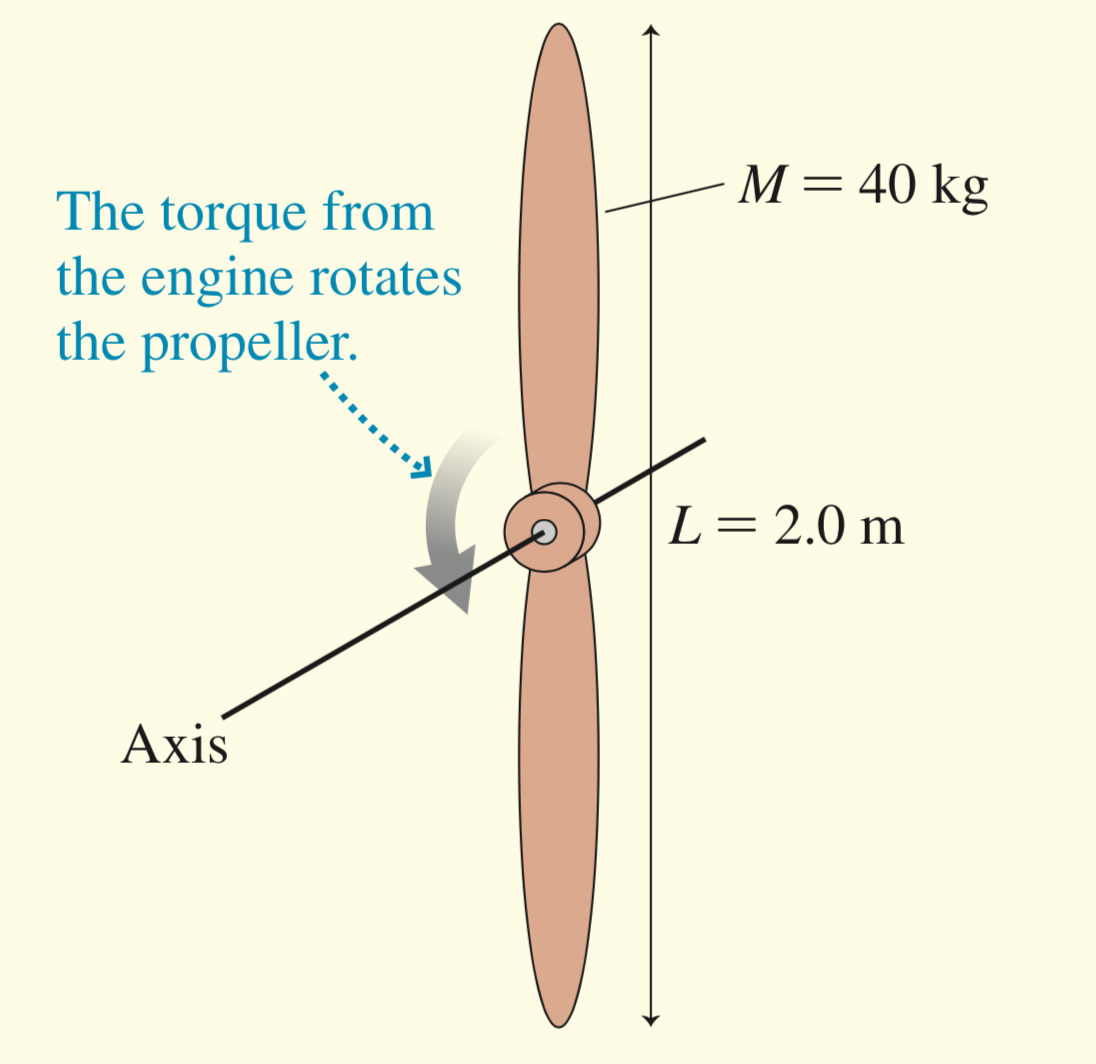
\includegraphics[width=.3\linewidth]{PS8_fig1}
	\caption{A rotating airplane propeller}
\end{figure}

The engine in a specified airplane is specified to have a torque of 60 Nm. This engine drives a 2.0-m-long, 40 kg propeller. On start-up, how long does it take the propeller to reach 200 rpm?


\end{document}
